%%%%%%%%%%%%%%%%%%%%%%%%%%%%%%%%%%%%%%%%%%%%%%%%%%%%%%%%%%%%%%%%%%%%%%%%%%%%%%%%
%2345678901234567890123456789012345678901234567890123456789012345678901234567890
%        1         2         3         4         5         6         7         8

\documentclass[letterpaper, 10 pt, conference]{ieeeconf}  % Comment this line out if you need a4paper

%\documentclass[a4paper, 10pt, conference]{ieeeconf}      % Use this line for a4 paper

\IEEEoverridecommandlockouts                              % This command is only needed if 
                                                          % you want to use the \thanks command

\overrideIEEEmargins                                      % Needed to meet printer requirements.

% See the \addtolength command later in the file to balance the column lengths
% on the last page of the document

% The following packages can be found on http:\\www.ctan.org
%\usepackage{graphics} % for pdf, bitmapped graphics files
%\usepackage{epsfig} % for postscript graphics files
%\usepackage{mathptmx} % assumes new font selection scheme installed
%\usepackage{times} % assumes new font selection scheme installed

%%%%%%%%%% my includes %%%

\usepackage{url}      % needed for ieeetran bib style
\usepackage{graphicx}
\graphicspath{{./03_graphics/}}

%checkmark
\usepackage{tikz}
\usepackage{pifont}% http://ctan.org/pkg/pifont
\def\checkmark{\tikz\fill[scale=0.4](0,.35) -- (.25,0) -- (1,.7) -- (.25,.15) -- cycle;} 
\newcommand{\xmark}{\ding{53}}%

% possible subfigure packages
%\usepackage{subfigure}
%\usepackage[caption=false,font=footnotesize]{subfig}

\usepackage[colorinlistoftodos, german]{todonotes} % Option 'disable' entfernt alle ToDos

\usepackage[utf8]{inputenc}

\usepackage[font=footnotesize]{caption}
\usepackage[font=footnotesize]{subcaption}
\newtheorem{thm}{Theorem}[section]
\newtheorem{defn}[thm]{Definition}


\usepackage{hyperref}

%% format tabular cells
\usepackage{booktabs}
\usepackage{tabularx}
\usepackage{makecell}
\renewcommand\theadalign{bc}
\renewcommand\theadfont{\bfseries}
\renewcommand\theadgape{\Gape[4pt]}
\renewcommand\cellgape{\Gape[4pt]}

%\usepackage[style=plain,citestyle=numeric,bibstyle=numeric,sorting=none,url=false,doi=false,isbn=false]{biblatex}

%%%%%%%%%%%%%%%%%%%%%%%%%%


\title{\LARGE \bf
Deep Reinforcement Learning with Continuous Control in CARLA
}

\author{Moritz Zanger$^{1}$ Florian Rottach$^{1}$ Izel Kilinc$^{1}$ % <-this % stops a space
\thanks{$^{1}$The authors are with FZI Research Center for Information Technology, Haid-und-Neu-Str. 10-14, 76131 Karlsruhe, Germany
%        {\tt\small \{kuhnt, zoellner\}@fzi.de}}%
        {\tt\small \{uvday, uydrn, uzdnz\}@student.kit.edu}}%
}        
        
\begin{document}



\maketitle
\thispagestyle{empty}
\pagestyle{empty}


%%%%%%%%%%%%%%%%%%%%%%%%%%%%%%%%%%%%%%%%%%%%%%%%%%%%%%%%%%%%%%%%%%%%%%%%%%%%%%%%
\begin{abstract}

%This electronic document is a ÒliveÓ template. The various components of your paper [title, text, heads, etc.] are already defined on the style sheet, as illustrated by the portions given in this document.

In the course of this project, three policy gradient reinforcement learning algorithms 
are implemented and evaluated using OpenAI Gym's CarRacing-v0 environment and the open-source 
urban driving simulator CARLA. To reduce sample complexity, four variants of input representations with 
differing dimensionalities are employed, of which the bird's eye view representation of ground truth 
segmented images delivers the best results. We can show that a top-down input representation is a feasible concept 
for a vehicle in a real-world scenario. As a result, we propose a reward function that enables stable 
lane-keeping behavior and smooth driving in CARLA.
\end{abstract}


%%%%%%%%%%%%%%%%%%%%%%%%%%%%%%%%%%%%%%%%%%%%%%%%%%%%%%%%%%%%%%%%%%%%%%%%%%%%%%%%
\section{Introduction}

%This template provides authors with most of the formatting specifications needed for preparing electronic versions of their papers. All standard paper components have been specified for three reasons: (1) ease of use when formatting individual papers, (2) automatic compliance to electronic requirements that facilitate the concurrent or later production of electronic products, and (3) conformity of style throughout a conference proceedings. Margins, column widths, line spacing, and type styles are built-in; examples of the type styles are provided throughout this document and are identified in italic type, within parentheses, following the example. Some components, such as multi-leveled equations, graphics, and tables are not prescribed, although the various table text styles are provided. The formatter will need to create these components, incorporating the applicable criteria that follow.

%Example Citation: \cite{Barth2008}.

The task of teaching vehicles how to drive autonomously in urban scenarios is a 
challenging and complex one to solve. Not only is there the problem of finding the adequate 
response to a given situation but also the challenge of taking into account the surrounding 
factors that have an influence on the state that a vehicle is in and its possible actions. 
To date, most approaches focus on the manual design of behavioral policies, such as defining a 
driving policy through the use of annotated maps \cite{7339478}. While these solutions might work in 
situations that are documented by the provided mapping infrastructure, they are often difficult to 
generalize or scale, as they do not necessarily enable the comprehension of any given local scene. 
In order to make autonomous driving truly feasible in a real-world scenario, it would be better to 
develop systems that can find their way without having to rely on an explicit set of rules. 
Reinforcement Learning methods provide one possible solution to this task. Here, the agent, 
i.e. the vehicle actively searches for the optimal driving policy while trying to maximize a 
numerical reward signal. As opposed to imitation learning techniques, which have been popular 
in finding driving policies \cite{kendall2019learning}, Reinforcement Learning algorithms enable 
a car to exceed human abilities, if applied correctly. In recent years, deep reinforcement learning 
methods have proven to be successful in solving complex tasks such as playing GO \cite{44806} or 
Atari \cite{mnih2013playing}, and there have been efforts in tackling various problems in the field 
of autonomous driving, including continuous control tasks \cite{lillicrapContinuousControlDeep2015}.

Two significant drawbacks of Reinforcement Learning methods are their heavy dependency on adequate 
input state representations \cite{DBLP:journals/corr/abs-1904-09503} and their imminent need for 
large amounts of data. In order to be able to 
train safely on an adequate amount of data, one approach is the use of data from other domains. For this purpose, 
the urban driving simulator CARLA has been developed, which is used as a simulation environment for this project.

In previous projects, CARLA has been used to learn policies that allow agents to navigate through complex urban 
environments with imitation learning methods \cite{DBLP:journals/corr/abs-1710-02410}\cite{DBLP:journals/corr/abs-1903-00640}. 
In this paper, it serves as an environment to solve a continuous control task via deep reinforcement learning. 
Several Reinforcement Learning algorithms are implemented and compared with regard to their 
performance, considering driving tasks of increasing complexity. Additionally, reward functions for the respective 
problems are tested, and different input representations are designed and evaluated.

%\subsection{Problem specification}
%\subsection{Why RL? What is our goal/motivation?}

\section{Related Work}

%1. Reinforcement learning tasks have been tackled successfully in the past
%	- discrete control tasks
%	- human performance could be "overcome"
%2. Continuous control is quite a new field
%	- Need different algorithms
%	- Adjustments and new developments have been made
%3. DDPG
%4. A3C
%5. PPO
%6. Autoencoder/DDPG
%7. Birds eye view
%8. CarRacing/TORCS
%9. We extend this to CARLA
%	- Has been done with imitation learning achieving good results
Various reinforcement learning tasks have been tackled successfully in the past, 
leading to notable advances in learning policies for simulated and real-world 
robotic control problems \cite{Levine:2013:GPS:3042817.3042937}\cite{Bruin2015TheIO} 
or solving complex game structures \cite{Schaul2015PrioritizedER}. The resulting Deep Reinforcement Learning
 methods have recently been developed so far as to achieving similar results or beating human 
 experts in some of these tasks \cite{44806}\cite{mnih2015humanlevel}. 
Silver et al. introduce a new approach of teaching an 
 agent the game of GO by combining Monte Carlo simulation with value 
 and policy networks to evaluate board positions and choose new moves. In autonomous driving, 
 Wolf et al. have achieved notable results using a Deep Q Network to evaluate possible steering 
 actions from an action space of five predetermined steering options \cite{7995727}. 

However, many tasks that could be solved with reinforcement learning approaches have 
continuous action spaces, to which approaches such as the DQN cannot be directly applied 
in a feasible manner \cite{lillicrapContinuousControlDeep2015}. Therefore, algorithms that 
can handle these high-dimensional action spaces have been developed in recent years. Mnih et al. 
present asynchronous variations of standard reinforcement learning algorithms and report the 
Asynchronous Advantage Actor-Critic (A3C) to have achieved the best results in their evaluations, 
including a physics control task with continuous action space in the MuJoCo Physics Simulator \cite{mnihAsynchronousMethodsDeep2016}. 
Lillicrap et al. introduce a different algorithm called Deep Deterministic Policy Gradient (DDPG), 
which they evaluate in simulated physical environments \cite{mnih2013playing}.

DDPG is also used by Kendall et al. to teach a full-sized autonomous vehicle a 
lane-following policy in an on-board manner. While already achieving good results 
with DDPG alone, they show that the additional use of a Variational Autoencoder dramatically 
improves the overall performance \cite{kendall2019learning}, suggesting an improved 
state representation as an area of possible further development in Reinforcement Learning 
for continuous control tasks. Another approach to reduce the complexity of visual 
features that has been investigated in several projects is the representation of the input 
images as a top-down view on the vehicle
 \cite{DBLP:journals/corr/abs-1812-03079}\cite{DBLP:journals/corr/abs-1903-00640}\cite{Djuric2018ShorttermMP}.

We extend this research by applying the aforementioned algorithms to autonomous driving tasks and evaluating their performance in OpenAI's CarRacing-v0 environment and in the CARLA driving simulator while investigating input states of differing complexity, such as bird's-eye view or latent space representations \cite{dosovitskiy2017carla}.

%“Human-level control through deep reinforcement learning” (2015)
%“CARLA: An Open Urban Driving Simulator”
%Our contribution to the field

\section{Background}

We regard the typical reinforcement learning setting where an agent interacts with an environment $\mathcal{E}$. At each one of a number of discrete timesteps $t$ the agent decides on taking an action $a_t$ from a given set of actions $\mathcal{A}$. This is done based on the state $s_t$ that the agent is currently in and following a policy $\pi$, which is a mapping of the possible states to the action space $\pi: \mathcal{S} \rightarrow \mathcal{P}(\mathcal{A})$. In this case, $\pi$ is stochastic, as it returns the probability distribution over the possible actions, and the action space is continuous.

As a result, the agent receives a reward $r_t$ and the subsequent state $s_{t+1}$ of his environment. The setup is assumed to follow the properties of a Markov decision process, where besides state space $\mathcal{S}$, action space $\mathcal{A}$ and reward function $r(s_t,a_t)$, we also include the transition function to the future states $p(s_{t+1}|s_t,a_t)$. The objective of the agent is to maximize his expected return $R_t$, which is the cumulative reward of the current state $s_t$ and the rewards of future states, discounted with a factor $\gamma \in [0,1]$.

In actor-critic methods the critic calculates the action value $Q^\pi(s,a) = E[R_t|s_t=s,a]$ describing the expected cumulative return for taking action a in state s under the given policy $\pi$, thus evaluating the selected action \cite{lilianweng}. The actor, on the other hand, estimates an optimal policy, following $\pi(s) = argmax_aQ(s,a)$. Similar to the action value, $V^\pi(s) = E[R_t|s_t=s]$ defines the value of state $s$ under the policy $\pi$ and describes the expected return for pursuing a policy $\pi$ from state $s$.

In our project, we consider a continuous control task in the context of autonomous driving where three different actions can be selected: steering in a range of [-1,1], throttle  and acceleration in a range of [0,1] respectively.

\section{Concept/Methods and Models}

In the course of this project, three different algorithms are used. Following the work of Lillicrap et al. \cite{lillicrapContinuousControlDeep2015} and Mnih et al. \cite{mnihAsynchronousMethodsDeep2016}, the DDPG and A3C algorithms are implemented and compared according to their performance in the Gym environment CarRacing-v0. Later on, the PPO algorithm is applied to solve a continuous control task in the CARLA simulator.

The concept for our project consists of four major fields of interest. 1. Evaluating the performance of the implemented algorithms in order to find the reinforcement learning model which resolves our task best. 2. Successfully defining a reward function that will teach the agent how to drive. Then, increasing the complexity of the reward function to driving in the right lane and, finally, driving in the lane without crashing. 3. Finding the optimal input state representation by varying the levels of realism of the input images. 4. Trying out the following three terminal conditions: Reaching more than 2000 steps, crashing and exceeding a certain distance to the center line of the road.
%TODO: Hier unser Konzept analog zur Präsentation vorstellen (Slide mit den 4 Kasten)
%\subsection{CarRacing - Understand and select algorithms}
%\subsubsection{Preprocessing}
%\subsubsection{DQN}

\subsection{DDPG}
One notable advance in reinforcement learning has been made by the development of the Deep Q Network (DQN) \cite{mnih2015humanlevel}. The DQN is able to solve tasks with high-dimensional observation spaces. However, it is only efficiently capable of working with discrete and low-dimensional action spaces. In order to adapt a DQN for the successful use with continuous control problems, as given in CarRacing-v0, a discretization of the action space has to be carried out, which can lead to two main difficulties: an explosion in the number of possible actions and the loss of important information \cite{lillicrapContinuousControlDeep2015}.

To evade these obstacles Lillicrap et al. propose a novel approach, the Deep Deterministic Policy Gradient, which is a model-free, off-policy actor-critic algorithm. They adopt the advantages of DQN and combine them with the actor-critic framework, resulting in the stabilization of Q-learning through the usage of a replay buffer and soft updates on the target networks $\theta'$ of both actor and critic, through

\begin{equation}
\tau << 1:\theta' \leftarrow \tau\theta + (1-\tau)\theta',
\end{equation}

as well as finding a deterministic policy.

In order to enable better exploration, we add noise in the form of the Ornstein-Uhlenbeck process to our policy. For our continuous control problem, we chose the Ornstein-Uhlenbeck process due to the fact that it produces temporally correlated noise, which enables smoother transitions, compared to e.g. Gaussian noise. 

\subsection{A3C}
The Asynchronous Advantage Actor-Critic (A3C), introduced by Mnih et al. \cite{mnihAsynchronousMethodsDeep2016}, has become a go-to algorithm in 
Deep Reinforcement Learning due to its performance, robustness, and ability to perform well on high-dimensional action and state spaces. 
A key characteristic of A3C is the utilization of multiple agents, each equipped with its own environment instance and its own set of network parameters. 
One of the advantages of this approach is the diversification of the collected experience but yields the challenge of handling gradient update 
mismatches between the asynchronously collected network parameter updates. 
In our implementation of A3C, we adapt several alterations as opposed to the original version by Mnih et al.. Despite being an on-policy method, we include a numerically efficient n-step return as proposed by jaromiru \cite{janischLetMakeA3C}. % (eq. x). 
% \begin{equation}
%    R_{0} = r_{0} + \gamma r_1 + \gamma^2 r_2 + ... + \gamma^{n-1} r_{n-1}
%    R_{1} = r_{1} + \gamma r_2 + \gamma^2 r_3 + ... + \gamma^{n-1} r_{n}
% \end{equation}
% With R denoting the discounted Return at each timestep, $\gamma$ the discount factor, and r the reward at each timestep. Rather than calculating 

Furthermore, experiences are buffered in a global update 
queue, and updates are only performed by a master network. This feature helps decorrelate experiences, emphasizes exploration, and allows for more GPU-friendly
batch-learning. However, one has to keep in mind that this contradicts the original update rule by Mnih et al. and might lead to policy lag. A proper update 
frequency in the master network is therefore of major importance.

\subsection{PPO}

The Proximal Policy Optimization (PPO) algorithm was developed to improve training stability by avoiding parameter updates that excessively change a given policy at each step. The algorithm that PPO is based on is called Trust Region Policy Optimization (TRPO) and realizes training stability through a KL divergence constraint on the policy update range at each iteration \cite{pmlr-v37-schulman15}. PPO simplifies this concept by incorporating the hard constraint into the objective function through Lagrangian duality and, thus, softening the constraint. Additionally, PPO clips the objective function if the ratio between old and new policy lies outside the range of [1-$\epsilon$, 1+$\epsilon$], which discourages large policy changes. Tests on benchmark tasks have shown PPO to achieve outstanding results while reducing TRPOs complexity significantly \cite{DBLP:journals/corr/SchulmanWDRK17}.

\subsection{Reward function}
The design of the reward function is of major importance to the outcome of this project while being a much more complex process than initially expected. In Gym's CarRacing environment, good results could be achieved in the end by employing the rather simple and already provided reward function to our model. For CARLA however, it was necessary to invest more time into the engineering and design of a suitable incentive system, as the driving behavior in this environment depends on a larger variety of factors and the performance is not only measured by the speed of the agent. IThe process of finding a suitable reward function comprises the following tasks: \newline 
In the first step, we investigate possible sensor and measurement inputs that might have an impact on the driving behavior and discuss their impact. As summarized in Table 1, the outcome consists of eight possible features that are subsequently tested.


\begin{table}[!h]
	\footnotesize
	\centering
	\caption{Identified reward function components}%
	\label{tab:Example}%
	\begin{tabularx}{\linewidth}{lcX}
		\toprule
		\textbf{Component} & \textbf{Description} & \textbf{Intention}\\
		\midrule
		\makecell[Xt]{Per frame penalty}  & \makecell[Xt]{The penalty amount subtracted from the reward for each frame}   & \makecell[Xt]{Forces agent to move in order to compensate the penalties}  \\
		\makecell[Xt]{Lane invasion increment}   & \makecell[Xt]{Is either 0 or 1 and reflects if a lane invasion took place for the current frame.} & \makecell[Xt]{The agent should perform as few lane changes as possible} \\
		\makecell[Xt]{Steering angle}   & \makecell[Xt]{The absolute angle of the steering wheel}       & \makecell[Xt]{Avoids oszillations in the driving behavior}   \\
		\makecell[Xt]{Delta heading}     & \makecell[Xt]{The angle between current street direction and car position}      & \makecell[Xt]{Agent should drive as straight as possible relatively to road direction} \\
		\makecell[Xt]{Position change}     & \makecell[Xt]{The angle between current street direction and car position}      & \makecell[Xt]{Maximize travelled distance} \\
		\makecell[Xt]{Collision binary per frame}     & \makecell[Xt]{Penalty for crashing into other vehicles, objects or road infrastructure}      & \makecell[Xt]{Avoid crashes and improve security of driving} \\
		\makecell[Xt]{Velocity}     & \makecell[Xt]{The agent's absolute speed retrieved from the CARLA engine}      & \makecell[Xt]{Forces the agent to move forward} \\
		\makecell[Xt]{Distance to middle lane}     & \makecell[Xt]{The absolute distance to center in meters - can also be squared to improve}      & \makecell[Xt]{Drive as centered as possible} \\
		\bottomrule
	\end{tabularx}
\end{table}


We start with incrementally adding these attributes to our reward calculation leading to the realization that the main challenge is adjusting the weights and harmonizing the contrary effects of the terms.
For example, giving the velocity a relatively high weight, such as 0.8, while giving the distance to centerline a weight of 0.2 results in an agent that speeds over the map and pays only little attention to lane invasions. On the other hand, the agent will drive very slowly or not at all, if the rewards for oscillations are too high compared to the velocity.Considering that we have not only two, but several possible components, this results in a complex combinatorial problem that can either be solved by trial and error or by applying permutational optimization techniques. Initial results are achieved by finding a reward function through the former method. 
\newline
The above list is reduced by applying the following considerations that result from testing different approaches. Firstly, some components show redundant behavior and, hence, one of them can be removed. An example would be the velocity and the position change - both contain the same information. Furthermore, the lane invasion and steering angle attributes do not affect driving behavior in a positive way. The two most important parameters turn out be the velocity and the delta heading, which expresses the relative angle to the current street angle. Our final reward function and the aggregation weights can be found in table 2.
\newline
We want to note here, that a performance-wise comparison between the different parameter combination is hard to measure with a metric and is not the aim of this project. However, it would make sense to develop a suitable approach to categorize and assess the performance of different reward functions towards the desired outcome. 

\begin{table}[!h]
	\footnotesize
	\centering
	\caption{Final reward function terms and weights}%
	\label{tab:Example}%
	\begin{tabularx}{\linewidth}{lcX}%
		\toprule
		\textbf{Component} & \textbf{Effect} & \textbf{Weight} \\
		\midrule
		\makecell[Xt]{Per frame penalty}   & \makecell[Xt]{Lead to a strong initial learning behavior. Already after few steps the agent kept accelerating to compensate this penalty.}  &\makecell[lt]{-0.01} \\
		\makecell[Xt]{Velocity}          & \makecell[Xt]{When selected too small, slow learning and when too high, strong lane oscillations / non-smooth driving.}  &\makecell[lt]{+0.05} \\
		\makecell[Xt]{Delta heading}          & \makecell[Xt]{Introducing this term improved the driving stability enormously.}  &\makecell[lt]{-0.005} \\
		\makecell[Xt]{Squared distance to middle lane}  & \makecell[Xt]{Squaring had very beneficial effects, other powers were to restrictive.}  &\makecell[lt]{-0.01} \\
		\makecell[Xt]{Collision binary}  & \makecell[Xt]{Might be set to an even higher value but lead to attempts to avoid other objects }  &\makecell[lt]{-100} \\
		\bottomrule
	\end{tabularx}
\end{table}

In combination with tuning the Reinforcement Learning models, the result is very promising and can be summarized as follows: The agent is capable of driving smoothly within the right lane and can perform turn maneuvers on most intersections. It attempts to drive around other vehicles but is not capable of braking. Different models were trained on this reward function and all of them had a good performance compared to other incentive attempts. We assume that even better results can be achieved by applying an improved optimization method to find the best parameter combination. However, this is a combinatorial problem and requires several simulation runs. 


\subsection{Input representation}
Dealing with the high-dimensional environment in CARLA is one of the central challenges in implementing a well functioning 
RL algorithm. In consideration of an abundance of possible sensor types available in CARLA we pursue increasing
levels of realism, which correspond to increasing levels of difficulty. The levels of realism involve the following:
\begin{itemize}
    \item Ground truth segmented bird's eye view
    \item Ground truth segmented front view
    \item Latent space generated from ground truth segmented images
    \item Latent space generated from RGB images
\end{itemize}
Notably, these input representations differ in dimensions and thus lead to different network architectures in the appended network architectures 
of the RL agent. 
\paragraph{Ground truth segmented bird's eye view}
The Ground truth segmented bird's eye view is a rather unrealistic scenario, in which we assume the availability of a camera positioned 
20m above the performing agent. It is merely imaginable in a fully observed city where autonomous driving is part of a high-level traffic 
control system. Though rather unrealistic, we implement a 13-class ground truth segmented bird's eye view due to its similarity to 
the CarRacing 
environment and its advantages in containing information central to navigational tasks. 
Dosovitskiy et al.\cite{dosovitskiy2017carla} describe the full list of the included classes in their original publication on CARLA. 
We deem a 1-channel 
grayscale image with size 64x64 
large enough to contain key information for the algorithm (Fig. 1. left).

\begin{figure}[thpb]
    \centering
    \framebox{\parbox{3in}{
    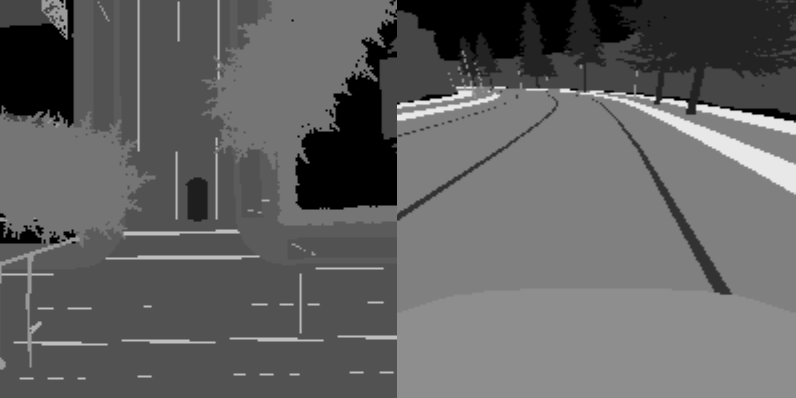
\includegraphics[scale=.271]{gt_combined.png}
    }}
    \caption{left: Ground truth segmented bird's eye view image, 64x64 in grayscale, 9 classes
    right: Ground truth segmented front view image, 80x80 in grayscale, 9 classes}
        \label{figurelabel}
        \end{figure}

\paragraph{Ground truth segmented frontview}
Much like the ground truth segmented bird's-eye view, the corresponding front view input representation assumes the availability of a 
perfect segmentation camera. Nonetheless, we increase realism with this representation as the camera is based on the car.
Again, we choose a 13-class, 1-channel grayscale image with a slightly increased size of 80x80 to account for a larger view angle of the 
camera. 
\paragraph{Latent space generated from ground truth segmented images}
We now further discuss a modified version of the integrated encoder-decoder network that is based on 
Dziubinski's \cite{dziubinskiSemanticSegmentationSemantic2019} implementation. 
The underlying idea of this model is to 
guide feature extraction towards more useful, problem-specific features by exposing the model to the additional 
target of reconstructing a bird's-eye view from the vehicle-based camera images.
In its original architecture, the network comprises 
five input tensors and seven output tensors with the inputs representing images of a front-, rear-, left-, right-, and top-view camera. The 
model is built with the Keras functional API and generally serves two purposes. On the one hand, each input tensor is encoded into 
a 64-sized feature vector and decoded into its original shape with a cross entropy loss with regard to the original input. This is 
achieved with separate branches of autoencoders with three convolutions, respectively. On the other 
hand, a separate generative branch creates a bird's-eye view reconstruction based on the concatenated feature vectors of the 
vehicle-based cameras. In addition to the cross entropy loss at the reconstructed bird's-eye view output, a mean squared error 
loss is calculated against the output of a subtract layer between the autoencoder's feature vector und the reconstructed feature vector to support
convergence. Notably, the autoencoder branch of the top-down camera view is solely purposed for improving the latent space of the generative branch 
during training and is thus not required for inference. 
\newline In comparison to Dziubinski's \cite{dziubinskiSemanticSegmentationSemantic2019} vanilla version, we 
adjust the architecture to fit the single camera bottlenecks into a length 64 vector and the reconstructed bird's-eye view
bottleneck into a length 128 vector. To reduce complexity, we condense both input and target segmentation images to three classes 
and implement a generalized weighted cross entropy\cite{zhangGeneralizedCrossEntropy2018} loss function to 
account for the unbalanced distribution of vehicles and obstacles.
\begin{figure}[thpb]
   \centering
   \framebox{\parbox{3in}{
   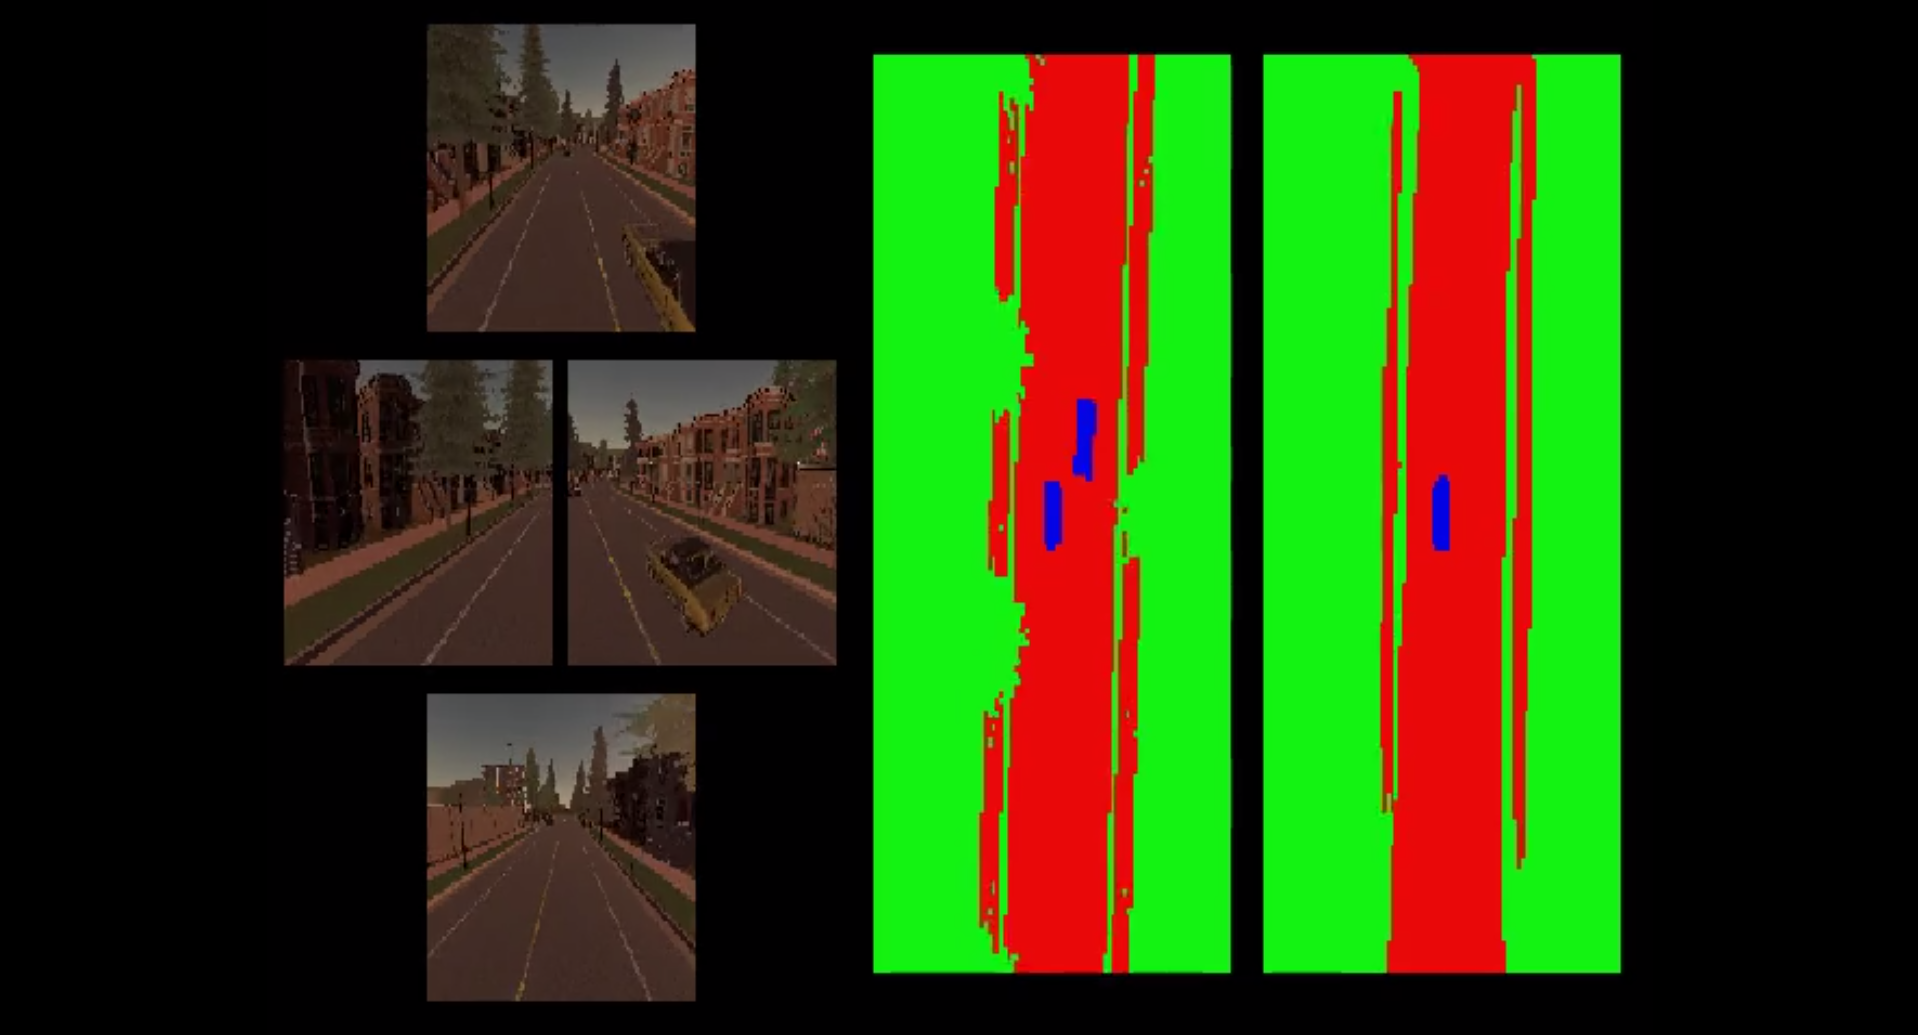
\includegraphics[scale=.113]{rgb_birdseye.png}
   }}
   \caption{left: RGB images from 4 vehicle-based cameras
            \newline 2nd from right: ground truth segmented bird's eye view
            \newline right: reconstructed bird's eye view}
       \label{figurelabel} 
       \end{figure}

\paragraph{Latent space generated from RGB images} To deal with the higher input complexity in RGB-images, we extended the
encoder and decoder models to 5 convolutions. Training data was collected both manually and by autopilot to retrieve a better 
balance in driving styles, speed and locations. During training, the maximum of 308 Vehicles were spawned in the environment to 
increase vehicle-class occurrence in the data. 
       
\subsection{Training}
In order to align the algorithms with the varying input dimensions, we had to implement a wrapper 
around the actual models that adjusts the network architecture accordingly. Especially the fact that 
the latent space is flattened and not 2-dimensional such as the ground truth pictures made it 
necessary to implement convolutional as well as  fully connected networks. 
Luckily, for the stable-baselines PPO model this is implemented very quickly. 
The architecture of our Keras-DDPG model however, had to be adjusted completely. 
We performed the training in four process steps, aligned with the input representation 
types mentioned previously. Therefore, the initial training was carried out on the ground-truth 
front view, afterwards on the ground-truth bird's eye view and finally we trained on the latent 
space of RGB and ground-truth segmented images. 
\subsubsection{DDPG}
The Deep Deterministic Policy Gradient performed well on our initial attempts within gym CarRacing 
and we identified reasonable hyperparameters for proper learning. We applied the same model 
on the new input features of CARLA and came to the sobering result that the input seemed to be 
too complex for the model. We assume that the learning algorithm was distracted by the advanced 
simulation environment. The following illustration emphasizes the poor behavior of the model 
(trained on circumstances where other models performed well). Hence, we decided to continue with 
different learning approaches and agreed due to recent developments on the PPO.
\begin{figure}[thpb]
	\centering
	\framebox{\parbox{3in}{
			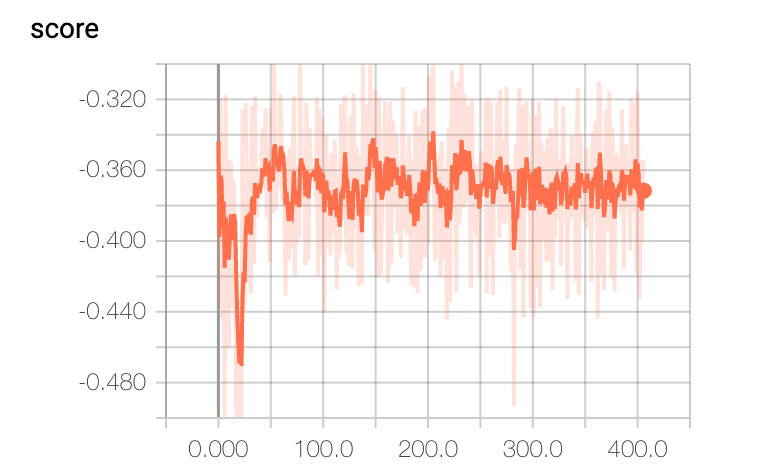
\includegraphics[scale=.5]{ddpg.png}
	}}
	\caption{Keras DDPG learning behavior}
	\label{figurelabel}
\end{figure}

\subsubsection{PPO}
The stable-baselines PPO2 model is easy to train and only few hyperparameters need 
to be adjusted. The drawback of this approach is that customization of these pre-defined 
models is rather laborious. Especially a combination of diverse input types such as scalars and 
images requires arduous architecture adjustments. We changed the following parameters and arrived 
at a very fast and crisp learning behavior that enables the agent to start driving after already very few episodes.

\begin{table}[!h]
	\footnotesize
	\centering
	\caption{Final reward function terms and weights}%
	\label{tab:Example}%
	\begin{tabularx}{\linewidth}{lcX}%
		\toprule
		\textbf{Parameter} & \textbf{Default Value} & \textbf{Selected Value} \\
		\midrule
		\makecell[Xt]{Learning rate}   & \makecell[Xt]{0.00025}  &\makecell[lt]{0.0004} \\
		\makecell[Xt]{Clip range}   & \makecell[Xt]{0.2}  &\makecell[lt]{0.1} \\
		\makecell[Xt]{Gamma}   & \makecell[Xt]{0.99}  &\makecell[lt]{0.97} \\
		\makecell[Xt]{N\_steps}   & \makecell[Xt]{128}  &\makecell[lt]{1024} \\
		\makecell[Xt]{Environment steps}   & \makecell[Xt]{25k}  &\makecell[lt]{200k} \\
	\end{tabularx}
\end{table}

The learning behavior usually increased until 200k steps and started to stagnate afterward. 
The achieved episode rewards and entropy loss over several runs were very stable and performance 
drops occurred rarely. The results on the proved input representations were very different: We trained 
the PPO with the same reward function, the same amount of steps at the same environment 
spawn point and hence assumed equal conditions. The front-cam-view resulted in a very 
oscillating driving behavior and the rewards were damped by the penalties for inaccurate delta heading. 
The birds-eye-view on the other hand had a very smooth driving behavior and deliverd the best performance in our test. 
This comes from the improved view on the street trajectory from above. 
Due to training capacity, we decided to restrict training to the feature vector of the RGB encoded model. Considering the easier and smaller latent 
space representation we realized that the algorithm trains very fast but can't reproduce the performance of the ground-truth. 


\begin{figure}[thpb]
	\centering
	\framebox{\parbox{3in}{
			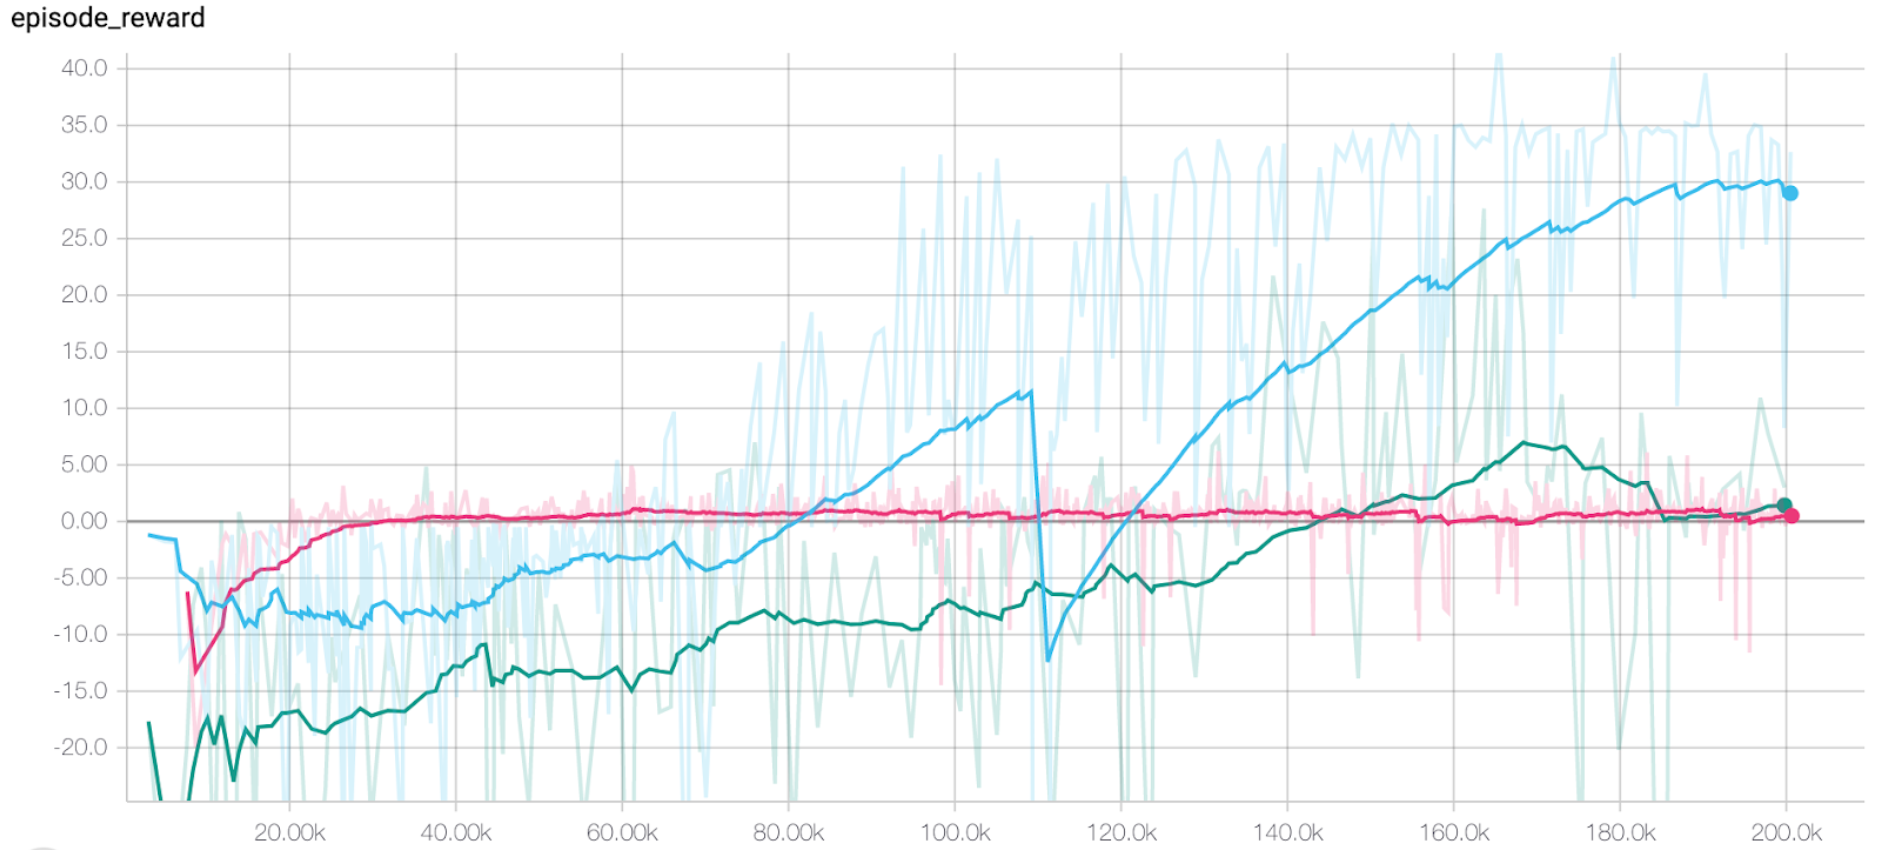
\includegraphics[scale=.23]{comparison_rewards.png}
	}}
	\caption{Green line: Performance on front-cam-view, Blue line: Performance on birds-eye-view, Red line: Performance on latent space of RGB model}
	\label{figurelabel}
\end{figure}


%\subsection{CARLA}

\section{Results}
\subsection{CarRacing-v0}
Due to the simple input structure and the straight-forward reward system, we achieved stable results, 
even with using not the most-advanced learning algorithms (We consider the PPO as an improvement over the DDPG). 
Also, the A3C could generate promising results (average rewards around 700) with only little training time.  
In total, these results can be explained by the simplicity of the environment. However, here we invested more time on 
the finetuning of the hyperparameters compared with CARLA.
\subsection{CARLA}
The CARLA simulation environment is far more complex than the previous environment we worked with. 
Since the application of the stable-baselines algorithms is rather straight-forward, the main challenge comprised the design of proper input 
representations and the optimization of terminal conditions, rewards and parameters.

\begin{table}[!h]
	\footnotesize
	\centering
	\caption{Project Goal: Input State Representations}%
	\label{tab:Example}%
	\begin{tabularx}{\linewidth}{lcX}%
		\toprule
		\textbf{Difficulty Level} & \textbf{Goal} & \textbf{Accomplished} \\
		\midrule
		\makecell[Xt]{Level 1}   & \makecell[Xt]{Ground truth segmented bird's eye view}  &\makecell[lt]{\checkmark} \\
		\makecell[Xt]{Level 2}   & \makecell[Xt]{Ground truth segmented front view}  &\makecell[lt]{\checkmark} \\
		\makecell[Xt]{Level 3}   & \makecell[Xt]{Latent space generated from ground truth segmented images}  &\makecell[lt]{discontinued} \\
		\makecell[Xt]{Level 4}   & \makecell[Xt]{Latent space generated from RGB images}  &\makecell[lt]{$-$} \\
	\end{tabularx}
\end{table}
As can be seen in TABLE IV, we were not able to produce a high-performance agent using the latent space of the RGB-model, 
despite its promising training speed. 
We assume that the architecture did not contain the complete information in the layers that were extracted in our
 experiment and that this was the reason, a similar outcome as the ground-truth birds-eye-view was not possible. One 
of the issues contributing to this, is the mismatch between the unconventional driving style of a learning agent and the 
driving style of a human/autopilot, at which data for the encoder-decoder model was collected. 
Despite using a weighted categorical cross entropy loss, the network struggled with reconstructing pixels
of the \textit{vehicle and obstacles} class. Aside from improving training data and network parameters, we consider the usage of more
sophisticated encoder-decoder models such as Deeplab-V3 for feature extraction as promising. Moreover, we believe feature extraction 
models should rather be fine-tuned during the agent's training, than be used for inference only. This way, a trade-off between 
problem-specific optimal feature extraction and data/time efficiency can be pursued. Given the variety of available sensors in CARLA, additional
input information such as 2D-Lidar data might further improve the agent's ability to avoid crashes. 

\begin{table}[!h]
	\footnotesize
	\centering
	\caption{Project Goal: Driving}%
	\label{tab:Example}%
	\begin{tabularx}{\linewidth}{lcX}%
		\toprule
		\textbf{Difficulty Level} & \textbf{Goal} & \textbf{Accomplished} \\
		\midrule
		\makecell[Xt]{Stage 1}   & \makecell[Xt]{Driving}  &\makecell[lt]{\checkmark} \\
		\makecell[Xt]{Stage 2}   & \makecell[Xt]{Lane Following}  &\makecell[lt]{\checkmark} \\
		\makecell[Xt]{Stage 3}   & \makecell[Xt]{Driving with Traffic and Obstacles}  &\makecell[lt]{\xmark} \\
	\end{tabularx}
\end{table}

TABLE V lists our overall project goals with respect to the driving behavior of our best-performing agent. 
The defined reward functions managed to teach our agent how to follow his lane with input states in ground truth bird's eye view representation.
The agent actively tried to avoid crashes in some cases, however, we believe that further adjustments to the reward function could improve 
the results in this area. Terminating after 2000 steps or after a crash improved the agent's behavior while terminating when the agent moved too far
from the center line had a negative impact on training results. 


\section{Conclusions}
As result of this practical seminar we have successfully applied different deep reinforcement 
approaches to the CARLA environment and finally achieved a stable and promising lane-keeping behavior 
for the agent. This was achieved by a combination of finding the most suitable input representation for 
smooth driving, finetuning of the rewardfunction and identification of the best performing hyperparameters. 
The outcome proves that reinforcement learning can be applied to complex environments as well as long as the 
desired behavior is incooperated in the reward system. Furthermore, we could prove that the birds-eye-view leads 
to a better performance as a single front camera and is also feasible in a real-world setup by generating the 
representation from four cameras surrounding the car. In the training process we recommend to not use early-termination 
for the episodes, especially if the reward function contains negative components, since this increases the probability that 
the agent starts to drive off the track as soon as possible. Finally, we emphasize that the driving behavior has the potential 
to be even further improved in the future by selecting better data, learning algorithms and an optimal reward function. 
We can also imagine, that the involvement of further attributes in the model such as the current velocity can be used 
to describe even more complex driving situations.  \newline
For the future we additionally suggest a combination of the birds-eye-view with a front camera 
in order to enable the identification of traffic signs and traffic lights, which wouldn't be 
possible from above. Also, we assume that the improvement of the encoder-decoder 
architecture could boost the learning speed and overall performance.



\addtolength{\textheight}{-12cm}   % This command serves to balance the column lengths
                                  % on the last page of the document manually. It shortens
                                  % the textheight of the last page by a suitable amount.
                                  % This command does not take effect until the next page
                                  % so it should come on the page before the last. Make
                                  % sure that you do not shorten the textheight too much.

%%%%%%%%%%%%%%%%%%%%%%%%%%%%%%%%%%%%%%%%%%%%%%%%%%%%%%%%%%%%%%%%%%%%%%%%%%%%%%%%



%%%%%%%%%%%%%%%%%%%%%%%%%%%%%%%%%%%%%%%%%%%%%%%%%%%%%%%%%%%%%%%%%%%%%%%%%%%%%%%%



%%%%%%%%%%%%%%%%%%%%%%%%%%%%%%%%%%%%%%%%%%%%%%%%%%%%%%%%%%%%%%%%%%%%%%%%%%%%%%%%

%References are important to the reader; therefore, each citation must be complete and correct. If at all possible, references should be commonly available publications.










\newpage
\bibliographystyle{IEEEtran}
\bibliography{IEEEabrv,04_mendeley-export/library}

\newpage

\appendices
\begingroup
\let\clearpage\relax 
\onecolumn 
\section{Appendix}
\begin{figure}[thpb]
	\centering
	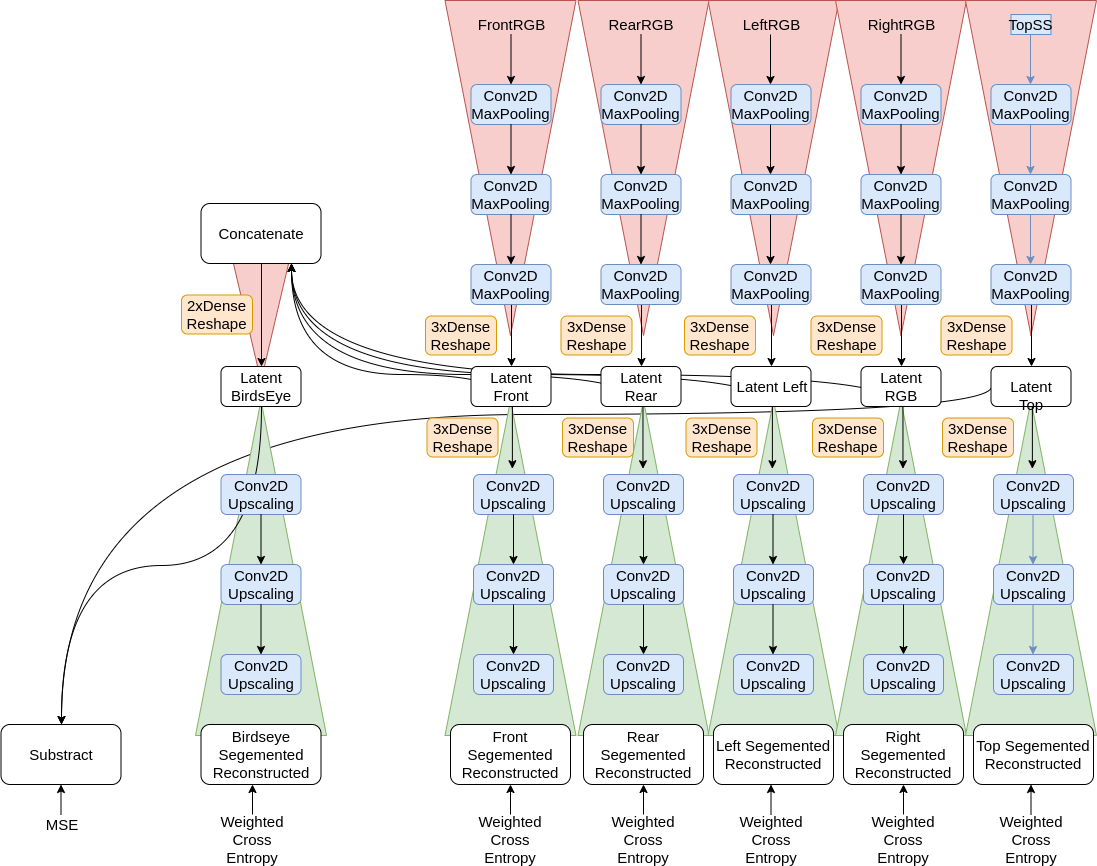
\includegraphics[scale=.35]{encoder_decoder_arc.png}
	\caption{Architecture of encoder-decoder model}
	\label{figurelabel}
\end{figure}
\begin{figure}[thpb]
	\centering
	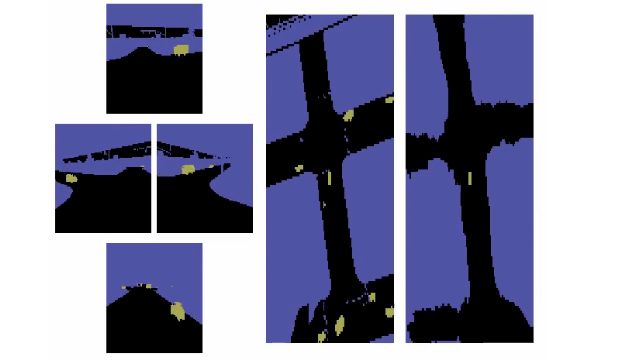
\includegraphics[scale=.5]{sem_reconstructed.png}
	\caption{Left: Four vehicle based ground truth semantic segmentation cameras \newline
	Center: Ground truth bird's eye view \newline
	Right: reconstructed bird's eye view}
	\label{figurelabel}
\end{figure}




\endgroup


\end{document}
